% Metoddelen redogör för vad du gjort och hur du gått tillväga; det är
% en beskrivning av den metod som ligger till grund för det du kommit
% fram till och hävdar i din rapport.

% Beskrivningen i metoddelen ska vara koncis snarare än helt
% uttömmande men ska samtidigt göra det möjligt att upprepa studien

% Metoddelen ska inte vara en omgjord labbinstruktion och den ska inte
% heller innehålla teori med mindre än att teoretiska hänsyn har haft
% en direkt inverkan på metoden.

% Metoddelen skrivs nästan alltid i dåtid (imperfekt) och ofta används
% passiv form för att beskriva forskningsaktiviteter.

\chapter{Metod}

\begin{draft}

Projektets genomförande bestod till störst del av konstruktionen av själva
läromaterialet, och där ingick skapandet av domänspecifika språk, skapandet av
den tillhörande lärotexten och publiceringen av denna på en hemsida. Därefter
följde en mindre del av utvärdering av materialet med en testgrupp som fick
svara på vad de tyckte om läromaterialet.

\section{Konstruktion av läromaterialet}

Läromaterialet består av ett antal kapitel som vardera behandlar separata
områden. Skapandet av varje kapitel skedde därför till största delen fristående
från andra kapitel. Skrivandet av alla kapitel bestod i sin tur av tre faser,
som såg likadana ut för alla kapitel. Dessa faser var val av område,
implementation av domänspecifika språk för området samt skrivande av lärotext.

Denna skapandeprocess kan delas upp i en graf med två axlar: en utefter kapitel och en
utefter fas. Det här illustreras i figur~\ref{fig:oversiktA}. Figuren visar att
varje kombination av kapitel och fas är en del i projektet som arbetades med.

\begin{figure}[tph]
    \centering
    \begin{subfigure}[t]{0.5\textwidth}
        \centering
        \frame{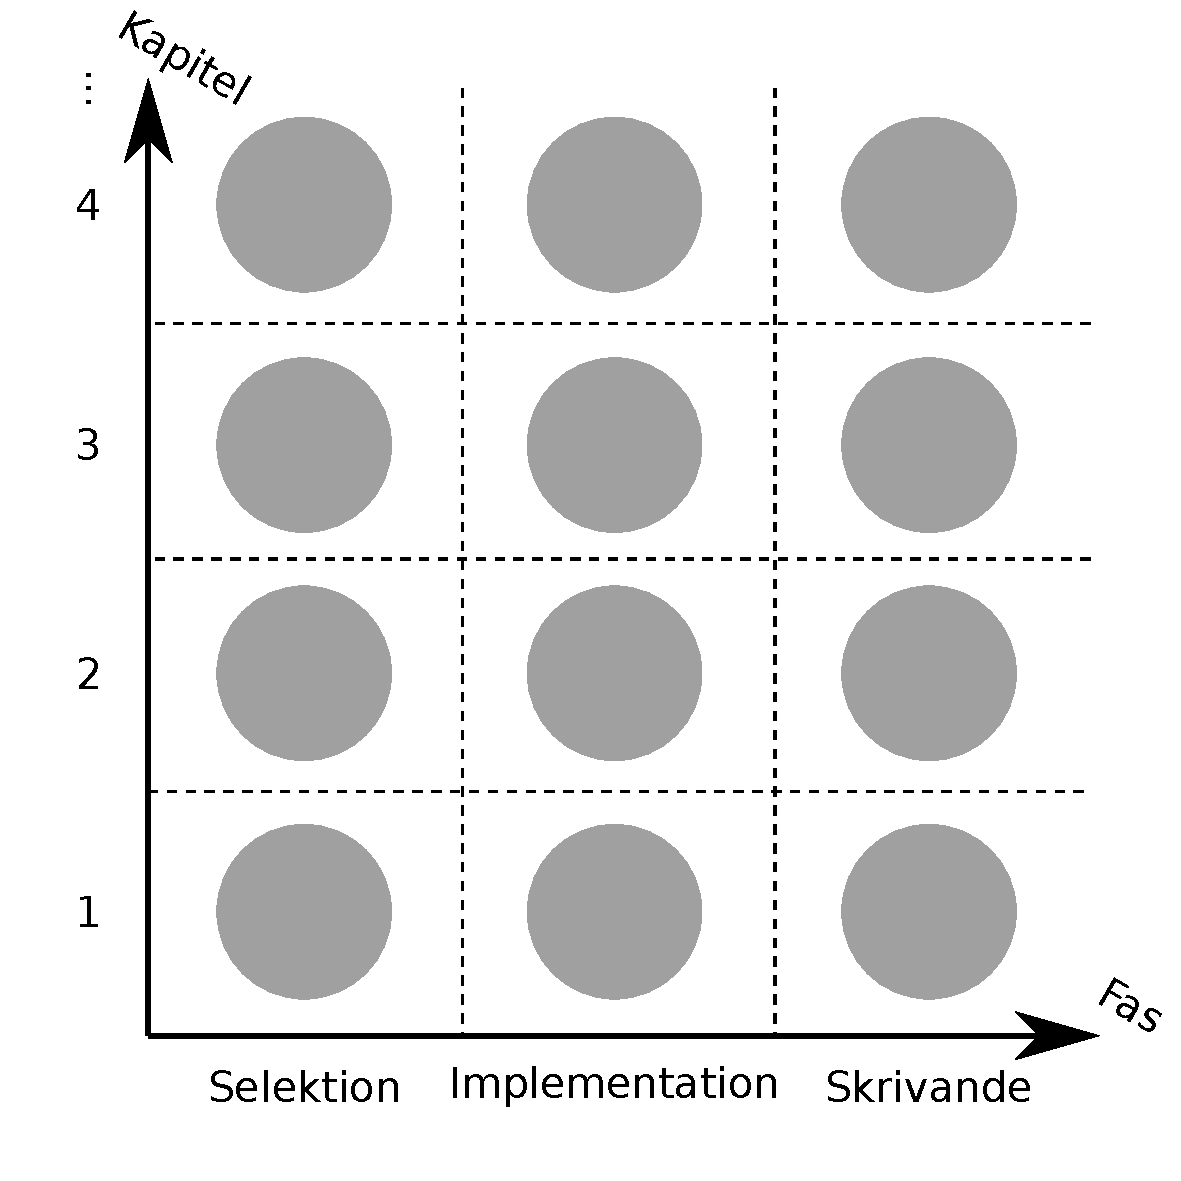
\includegraphics[width=0.9\linewidth]{figure/oversiktA.pdf}}
        \caption{Delarna visas distinkta och var för sig.}\label{fig:oversiktA}
    \end{subfigure}% <- This comment makes the figure lie side by side ¯\(°_o)/¯
    ~
    \begin{subfigure}[t]{0.5\textwidth}
        \centering
        \frame{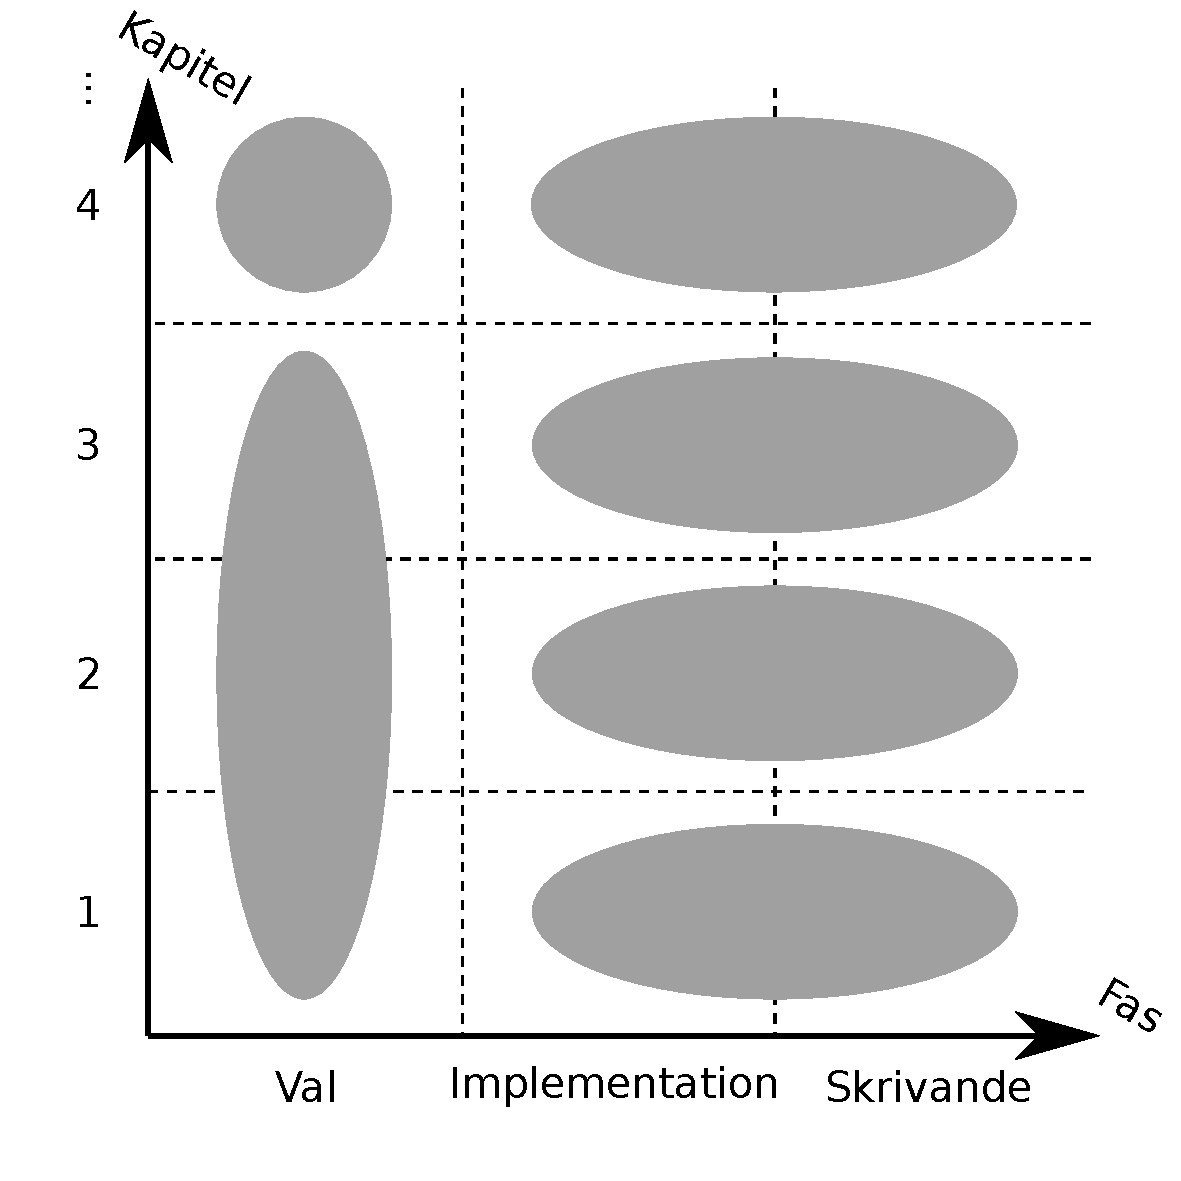
\includegraphics[width=0.9\linewidth]{figure/oversiktB.pdf}}
        \caption{Delarna visas med gränsöverskridande överlapp. Notera att
        implementation och skrivande \textit{alltid} var överlappande medan
      selektion \textit{ofta men inte alltid} var det.}~\label{fig:oversiktB}
    \end{subfigure}
    \caption{Översikt över hur skapandeprocessen av läromaterialet såg ut.
  Processen delas upp utefter två axlar: kapitel och fas. Varje kombination
  är en del som arbetats med och är gråmarkerad.} \end{figure}

Även om detta sätt att dela upp processen är översiktlig är den inte helt
verklighetstrogen. I praktiken fanns det överlapp mellan de olika delarna, både
med avseende på kapitel och fas. Det här illustereras i
figur~\ref{fig:oversiktB}. Där ser man att valet av områden skedde för flera
kapitel samtidigt. Detta då arbetet med att hitta ett områden ofta gav flera
områden samtidigt. I figuren ser man också att implementation av domänspecifika
språk och skrivande av lärotext skedde samtidigt. Eftersom de i resultatet är
sammanvävda är det också högst naturligt att processerna med att skapa dem
också var sammanvävda.

De tre följande avsnitten beskriver i detalj hur de tre faserna, val,
implementation och skrivande såg ut. Det är viktigt att minnas att det, som
nämndes ovan, finns överlapp mellan både faserna och kapitlena.

\subsection{Val av områden att behandla}\label{sec:valet}

Ett domänspecifikt språk modellerar ett specifikt och avgränsat område. Därför
var det naturligt att söka och tänka i termer av avgränsade områden inom
fysiken. För att mer konkret hitta områden att behandla kontaktades Åke Fäldt,
examinator för \textit{Fysik för ingenjörer}\todo{Ref?}, samt att studera fysikkursens
bok, \textit{Univeristy Physics}\todo{Ref?}.

Fäldt befrågades om vilka områden han i allmänhet anser studenter har
svårt för. Detta för att i enlighet med projektets mål börja med de, för
studenterna, problematiska områdena. Enligt Fäldt är ett allmänt problem att
egna mentala modeller för problem är felaktiga eftersom studenter ofta tar
genvägar som inte bygger på saker de är säkra gäller. En annan erfarenhet
från honom är att så länge första raden i en uppgiftslösning är rätt, så är
resten också rätt. Med andra ord, har studenten väl identifierat vilken typ av
problem det rör sig om brukar det inte vara några svårigheter att lösa
uppgiften.

Med hjälp av insikterna från Fäldt drogs två slutsatser. Den första slutsatsen
var att matematisk analys var ett område värt att behandla i detalj. Den andra
slutsatsen var att genom att ge struktur till olika typer av problem kan det
förhoppningsvis underlätta för studenter att lära sig att identifiera vilken
typ av uppgift de handskas med.

Ett inledande val gjordes för att hitta mer specifika områden att arbeta.
Detta genom att studerade kursboken \textit{University Physics}.
Speciellt av intresse var de kapitel som behandlade mekanik (i enlighet med
projektets mål att börja med klassisk mekanik), matematisk analys samt de
kapitel som använde sig av en specifik syntax \todo{Syntax?}. Domänspecifik
syntax var av intresse att finna då en betydlig del av domänspecifika språk är
modellering av just syntaxen. \todo{Kanske förtydliga/utveckla varför detta är
av intresse} Även områden som projektgruppen fann personligen intressanta,
valdes ut.

Allteftersom arbetet fortskred blev det tydligt att det fanns en distinktion
mellan \textit{grundläggande} och \textit{komposita} områden.  Där de
grundläggande områdena var områden som inte var beroende på andra delar inom fysiken
utan kunde implementeras helt fristående från varandra. Till skillnad från de
komposita områdena vilka byggde vidare på de grundläggande områdena och/eller andra
komposita områden.

\end{draft}

\subsubsection*{Grundläggande områden}

\begin{binge}

\textbf{Fortfarande inte helt nöjd med detta avsnitt, känns som att det kan vara
lite otydligt och upprepande}

Grundläggande områden hittades främst genom det tidigare nämnda inledande
valet av områden (se avsnitt~\ref{sec:valet}). Detta eftersom litteraturen som
studerades började med just dessa områden för att sedan bygga vidare på dem i
mer avancerade kapitel.

Fler grundläggande områden har också hittats i efterhand. Avslutande av den
inledande inläsningen innebar alltså inget stopp av sökandet av grundläggande
områden, även om de flesta redan hittats. Fler grundläggande områden hittades
bland annat även genom att studera kursmaterialet som tillhörde \textit{Fysik
för ingenjörer}.

Sökandet i kursboken och kursmaterialet gav viktiga kunskaper om områden att
behandla. Men minst lika viktiga var de experiment som gjordes för att se
huruvida ett område lämpade sig som ett grundläggande område. De områden som inte
lämpade sig fick istället behandlas annorlunda (se `Komposita områden'' nedan). 

Förenklat sagt var de områden som innehöll tydlig data och tydliga operationer väl
lämpade som ett grundläggande område. Lämpligheten hos olika områden diskuteras
utförligare i avsnitt~\ref{sec:lampligt}.

När de grundläggande områdena valdes ut definerades de så att det i största möjliga
utsträckning var fristående. Detta för att kunna arbetas med parallellt. De
grundläggande områdena som under projekets gång valdes ut blev bevis,
dimensioner, matematisk analys och vektorer. 

\textbf{OCH FLER?}
\end{binge}

\begin{draft}
\textit{Bevis} eftersom det ger en insikt i hur de formler man använder
faktiskt uppstår. För att genomföra bevis krävs också att formler och
beteckningar görs rigorösa, vilket ger en bättre förståelse av dem.

\textit{Dimensioner} eftersom det är viktigt för studenter att förstå sig på
hur dimensioner påverkas av algebraiska operationer. Det kan också vara
hjälpsamt att kunna utföra automatisk, datorassisterad dimensionsanalys på
beräkningar.

\textit{Matematisk analys} eftersom alla koncept i klassisk mekanik är
relaterade genom matematisk analys. Mer specifikt används differenser för att
beskriva medelrörelse, och infinitesimalkalkyl för att beskriva
momentanrörelser. Vidare var infinitesimalkalkyl just det område som Fäldt
pekade ut som speciellt viktigt och något som studenter har svårt för.

\textit{Vektorer} eftersom det är en viktig grundsten inom den klassiska
mekaniken. Alla krafter, hastigheter och accelerationer betraktas som vektorer i
planet eller rummet, och dessa är alla fundamentala element inom klassisk
mekanik.
\end{draft}

\begin{binge}
\textbf{OCH FLER?}
\end{binge}
  
\subsubsection*{Komposita områden}
\begin{draft}
Komposita områden identifierades då det framgick att området var en
vidareutveckling och/eller kombination av redan behandlade områden. Lösningen
blev därför att tillämpa redan skrivna domänspecifika språk för att modellera
dessa.

Ett sätt som komposita områden hittades var därmed som ett resultat av sökandet och
experimenterandet med grundläggande områden. Ett annat sätt var att även
komposita områden direkt söktes efter. Då användes precis som tidigare nämnts
främst kursboken och kursmaterialet tillhörande \textit{Fysik för ingenjörer}.
\end{draft}
\begin{binge}
\textbf{Är detta tydligt nog?} 

Ett exempel på ett komposit område är momentan- och medel-rörelse eftersom det
direkt utgör en stor delmängd av alla problem inom mekanik i \textit{Fysik för
ingenjörer}. Väldigt många av de uppgifter studenter lär sig lösa inom mekanik
är sträcka/hastighet/acceleration/kraft problem. Hur lång tid tar det att åka
en sträcka om man har en viss medelhastighet? Om ett objekt med massa $m$
påverkas av en kraft som varierar enligt $\sin(t)$, vad är då
momentanhastigheten vid $t=10$? Detta är en kombination av det grundläggande
området som behandlar vektorer och området som behandlar matematisk analys.
\end{binge}

\subsection{Implementation av DSL för områdena}
\begin{binge}
\textbf{FRÅGA: Är det tydligt vad som menas med experimentering?}

Implementationen av ett domänspecifikt språk till ett område inleddes med
experimentering. Även om en del experiment redan gjorts under urvalsfasen 
behövdes mer göras \todo{Motivera eller diskutera}. Det finns ingen absolut
kanonisk form \todo{förklara kanonisk form} att skriva ett domänspecifikt språk
på, framförallt inte för fysik \todo{Varför är det framförallt för fysik?}.
Experimentering var därför viktigt för att finna lämpliga representationer av
syntax och andra element av domänspecifika språk.

Framförallt eftersom vi inte vet hur den kanoniska formen ska se ut, det finns
ingen almänn bestämd form. Och det är också det som är motivationen till vårt
projekt. Nåt om paperet. \todo{Utveckla och skriv om}

Vad som ansågs vara en bra, eller åtminstone tillräckligt bra, representation
var i huvudsak baserat på gruppmedlemmarnas intuition om Haskell och diskussion
inom gruppen och med handledaren. Implementationerna skulle vara både
naturliga, i den mening att de gick att använda smidigt rent tekniskt. Men de
skulle även vara lättförståliga. Den progamtekniskt elegantaste
implementationen användes därför inte alltid, utan den mer verbosa versionen
föredrogs för att göra läromaterialet så lättläst som möjligt. Dock avstod vi
inte från de mer avancerade funktionerna i Haskell när de var motiverade av
materialet som vi beskrev, men då alltid med en utömmande förklaring av hur det
fungerade och utan krav på tidigare kunskap hos läsaren.

De olika områdena krävde i varierande mån inläsning och studering av Haskell,
fysik, matematik och domänspecifika språk. Till exempel krävde kapitlet om
dimensioner inläsning om typnivå-programmering i Haskell. 

HÄR BEHÖVER JAG HJÄLP ATT EXPANDERA JOHANS STYCKEN

I allmänhet implementerades DSL i Haskell som en kombination av syntaxträd,
funktioner för att manipulera dessa träd, och evalueringsfunktioner till något
slags semantisk domän\todo{Vad är ett semantiskt domän}. Komposita DSL var
istället mer \todo{beskrivning}. Varje DSL, grundläggande och komposita,
parades även ihop med en mängd fysikproblem att appliceras på, sådant att
läsaren skulle få förståelse för hur DSLen kan brukas utöver hur de
implementerades.

\textbf{TODO: En generell beskrivning av implementation}

\textbf{TODO: Ett specifikt exempel på implementation}

Syntax analyserades och modellerades i syntaxträd. För vissa områden
(enheter?) definierades även ett semantiskt värde som representerade
en slags kanonisk form.

För vektorer gjordes ...

För enheter gjordes ...

För analys gjordes ...

För annat gjordes ...

Efter att ett domänspecifikt språk implementerats skrevs tester till det. Det som var intressant att testa var olika lagar som skulle gälla. Eftersom de domänspecifika språk modellerade matematik var det matamatiska lagar som skulle gälla. Ett exempel är att vektoraddition skulle vara kommutativ.

Testerna gjordes med hjälp av \textit{QuickCheck}. QuickCheck är ett testningsverktyg i Haskell som genererar många och slumpmässiga testfall. Att lagarna gällde för de domänspecifika språken verifierades med andra ord genom testa för många exempelvärden. Inga bevis av att lagarna gällde gjordes.

\textbf{Saker som vi väntar en stund med att skriva}

KOMPOSITA ASPEKTER

Till de komposita områdena implementerades inga domänspecifika språk. Istället användes de tidigare språken som skapats för de grundläggande områdena. SKRIV MER HÄR NÄR VI GJORT NÅGRA KOMPOSITA

Importera DSLerna för varandra för att göra mer komplicerade grejer.

Eller, \emph{Bruk av de mer fundamentala/teoretiska DSLerna för att
  angripa områden av mer ``tillämpad'' natur (såsom Krafter, Arbete,
  etc) )}(?)

\subsection{Skriva lärotext}

I samband med att ett område implementerades skrevs också den tillhörande
lärotexten. Till en början skrevs lärotext som fokuserade på att förklara
programkoden. Detta var ett naturligt val eftersom det var viktigt att
programkoden gick att förstå innan kopplingar till matematik och fysik kunde
förklaras. Det var nämligen lärotext av det slaget som skrevs senare.
Avslutningsvis skrevs inledning och avslutning till kapitlet.

Generellt under skrivningen av lärotext togs det hänsyn till ARCS som
presenterats i avsnitt~\ref{sec:arcs}. 

\textbf{TODO: skriv mer här när vet om ARCS.}

Lättsamt språk och en gnutta humor för att hålla kvar
uppmärksamhet. Relaterat till Attention i ARCS modellen (2016
använde den. Såg vettig ut).

TODO: Expandera. Vad exakt använder vi för didaktisk metod? Samma
som appliceras i Learn You a Haskell, mer eller mindre. Fånga
uppmärksamhet med lite humor och lättsamhet etc.

Lärotexten och programkoden skrevs sammanvävt i samma fil, i \textit{Literate
Haskell}, se avsnitt~\ref{sec:lhs}. Literat programmering passade bra ihop med
hur läromaterialet skulle se ut då det betonade det jämnbördiga förhållandet
mellan programkod och förklaringar. För att läromaterialet skulle vara
lättförståeligt var det också viktigt att presentera materialet i den ordning
som en mänsklig läsare, och inte datorn, tyckte var enklast.\todo{I Quantity så
är detta tydligt. Då gjordes en ''taste of types'' tidigt för att läsaren
skulle förstå Quantity bättre, innan massa detaljer gicks in på. Frågan är dock
om detta ska gås in på i rapporten?}

\textbf{TODO: Skriva om övningar.}

KOMPOSITA ASPEKTER

Vari vi visar att DSLerna både är praktiskt användbara, likt Wolfram
Alpha, och att implementationen+applikationen hjälper oss förstå
mekanik i allmänhet och probleminstanserna i synnerhet.

\section{Skapande av och publicering på hemsidan}

  Läromaterialet publiceras på en internethemsida, varpå man kan läsa
  allt o ha skoj.

  TODO: Slå ihop underrubriker till ett stycke.

  \subsection{Beskrivning}

  Ett build-script hämtar .lhs källfilerna, i vilka lärotexten är
  skriven med markdown. Rendrar med pandoc, och sätter in lite
  navigationselement etc. med hjälp av eget templating-system. Manuellt
  läggs sedan stoffet på gh-pages branchen för att automatiskt visas på
  dslsofmath.github.io/BScProj2018. \todo{Förklara templating, rendrar, branch}

  Obs: Medan bygget är scriptat så är inte publiceringen det, och
  ingenting genereras/publiceras automatiskt kontinuerligt. Måste köra
  scriptet manuellt och lägga stoff på gh-pages branchen.

  \subsection{Build-script}

  I.e. implementation av python-build-scriptet i mer detalj.

  TODO: Är detta ens intressant? Viktigt för att producera sidan såklart, men
  inte intressant ur varken matte eller haskell/DSL perspektiv.

  \subsection{Hemsidan}

  TODO: Nåt om design, läslighet, grafik(?), navigation, avsiktligt undvikande
  av javascript, etc.

Från resultat: ska integreras här

Hemsidan består av grundläggande HTML, CSS och javascript. På hemsidan finns en innehållsförteckning med klickbara länkar till de olika kapitlen. Hemsidan är öppen för alla och bör fungera i de flesta webläsare. Javascript är inget krav för hemsidan. Matematiska formler visas ändå, om än inte lika tydligt.

  \section{Test och återkoppling}

  % Återkoppling från examinator (NAD): "Nils Anders Danielsson <nad@cse.gu.se>
  % 27 Feb (1 day ago)
  % to Patrik, Andreas
  % Hi,Your BSc project groups both try to make tools for learning. I had some
  % discussion with Andreas' group about their plans for evaluating how well
  % their product works. My position is that, given the resource limits of
  % these projects (and general problems of reproducibility in social
  % sciences), it is very hard to perform an evaluation that gives useful
  % results. I don't mind if your groups try to perform some kind of
  % evaluation, but I suggest that you tell them to avoid overstating the
  % importance of the evaluations in the final reports."
  % Jag tror det är kompatibelt med det jag sagt tidigare - att göra en "ordentlig" utvärdering av det pedagogiska utfallet är komplicerat och tar (kalender-)tid.
  % Informell utvärdering av en testgrupp bör dock ingå.

  Test på försöksstudenter. Återkoppling med Åke(?).

  Nog bra att vara explicit här med att det inte är en rigorös empirisk
  studio, om inte det redan täckts väl i Avgränsningar.

\end{binge}
